\maketitle
\tableofcontents
\newpage
\section{Theorie}
\label{sec:theorie}
Zentrales Thema des Versuchs ist Ultraschall. Dieser liegt ungefähr im Frequenzband von
\SI{20}{\kilo\hertz} bis \SI{1}{\giga\hertz}. Unterhalb dieser Frequenz, von \SI{16}{\hertz}
bis \SI{20}{\kilo\hertz}, liegt der menschliche Hörbereich. Oberhalb der Frequenz von Ultraschall gibt
es noch den Hyperschall und unterhalb des menschlichen Hörbereichs den Infraschall. Schall
lässt sich darstellen als longitudinale Welle
\begin{equation}
    \rho (x, t) = \rho_0 + v_0 \, Z \, \symup{cos} (\omega t - kx)
    \label{eqn:1}
\end{equation}
mit $Z = c \cdot \rho$ als akustische Impedanz, die abhängig ist von der Dichte
$\rho$ des Materials und der materialabhängigen Schallgeschwindigkeit $c$.
Durch Absorption verliert die Schallwelle bei der Ausbreitung Energie. Beschreiben
lässt sich dies durch die exponentielle Abnahme der Intensität $I$
\begin{equation}
    I(x) = I_0 \cdot \symup e^{-\alpha x} \, .
    \label{eqn:4}
\end{equation}
Dabei fällt die Intensität nach der Strecke $x$ exponetiell mit dem Absorptionskoeffizienten
$\alpha$ ab. Dieser ist zum Beispiel für Luft sehr groß, sodass in der Medizin ein Ultraschallgel
als Medium zwischen Ultraschallsender und Material genutzt wird.

Außerdem wird ein Teil der Schalwelle reflektiert, sobald diese auf eine Grenzfläche trifft.
Das Verhältnis aus reflektierter und einfallender Intensität wird als Reflexionskoeffizient
$R$ bezeichnet.


Erzeugt werden kann Ultraschall unter Zuhilfenahme des piezo-elektrischen Effekts.
Ein piezoelektrischer Kristall, meist ein Quartz, wird duch ein sich periodisch änderndes elektrisches Feld
zu Schwingungen angeregt und strahlt dadurch Ultraschallwellen ab. Stimmt die Frequenz des
elektrischen Wechselfeldes mit der Eigenfrequenz des Kristalls überein (liegt also ein
Resonanzfall vor),
erreichen die abgestrahlten Ultraschallwellen hohe Amplituden und damit auch hohe Energieichten.
Der piezo-elektrische Effekt lässt sich umkehren und somit lassen sich die
Kristalle auch als Schallempfänger nutzen. Einlaufende Schallwellen regen den Kristall dabei zu Schwingungen an.

Häufig werden in der Medizin Laufzeitmessungen mittels Ultraschall durchgeführt,
um an Informationen zu gelangen. Dabei gibt es zwei Verfahren:
\begin{itemize}
  \item \textbf{Durchschallungsverfahren}
  Bei diesem Verfahren befinden sich Sender und Empfänger gegenüber voneinander.
  Dazwischen befindet sich das zu durchschallende Material. Bei einer Fehlstelle
  in der Probe wird die Intensität abgeschwächt. Im Gegensatz zum Impuls-Echo-Verfahren
  ist keine quantitative Aussage darüber möglich, vgl. Abbildungen \ref{fig:1} und \ref{fig:2}.
  \begin{figure}{h}
    \centering
    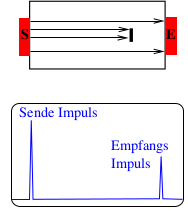
\includegraphics[scale=0.5]{durchschall.png}
    \caption{Das Prinzip des Durchschallungsverfahren \cite{anleitung}.}
    \label{fig:1}
  \end{figure}

  \item \textbf{Impuls-Echo-Verfahren}
  Im Gegensatz zum Durchschallungsverfahren fungiert hier der Sender auch als Empfänger.
  Dabei kommt zum Tragen, dass Schalwellen an Grenzwellen teilweise reflektiert werden (siehe oben).
  Mit diesem Verfahren können Fehlstellen bestimmt werden, so kann man aus der
  Höhe des Echos auf die Größe der Fehlstelle schließen. Außerdem kann mithilfe der Formel
  \begin{equation}
    s = \frac{1}{2} c \, t
    \label{eqn:6}
  \end{equation}
  bei bekannter Schallgeschwindigkeit $c$ und Zeit $t$ die Position $s$ der Fehlstelle bestimmt werden, siehe Abbildung \ref{fig:2}.
  Für die Darstellung der Laufzeitmessung gibt es den A-Scan, B-Scan und TM-Scan. Beim A-Scan wird die Amplitude
  gemessen (A: Amplitude), beim B-Scan wird die Amplitude in Helligkeit (B steht für Brightness) umgewandelt und
  beim TM-Scan wird die Amplitude gegen die gegeneinander verschobenen Echozüge von hintereinander liegenden Impulsen aufgetragen (TM: time motion).
  \begin{figure}
    \centering
    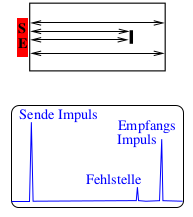
\includegraphics[scale=0.5]{impuls.png}
    \caption{Skizze des Impuls-Echo-Verfahrens \cite{anleitung}.}
    \label{fig:2}
  \end{figure}
\end{itemize}
\section{Durchführung}
\subsection{Versuchsaufbau}
Der Aufbau des Versuchs besteht aus Ultraschallechoskop, einer Ultraschallsonde mit
\SI{2}{\mega\hertz} und einem Rechner mit dem Programm EchoView, um die Daten darstellen zu können.
Am Echoskop lässt einstellen, ob eine (Impuls-Echo-Verfahren) oder zwei (Durchschallungsverfahren, siehe Kapitel \ref{sec:theorie})
Ultraschallsonden verwendet werden. Außerdem lässt sich eine Verstärkung in \si{\decibel} und
der TGC, ein zeitabhängiger Verstärkungsfaktor, (TGC: Time Gain Control, auch in \si{\decibel}) wählen. Als Untersuchungsmaterial stehen verschieden lange Acrylzylinder und
- platten, ein Augenmodell und als Kontaktmittel bidestilliertes Wasser zur Verfügung.
\subsection{Versuchsdurchführung}
Zuerst werden einige Testmessungen durchgeführt und probeweise die Schallgeschwindigkeit
bestimmt. Diese Messungen werden aber im Folgenden nicht weiter behandelt. Danach wird
das Impuls-Echo-Verfahren angewandt. Zu diesem Zweck wurden alle Acrylzylinder mit einer
Schieblehre mit einer Genauigkeit von \SI{0.2}{\milli\meter} vermessen. Als nächstes
werden Zylinder und Ultraschallsonde mit bidestilliertem Wasser gekoppelt.
Mittels eines A-Scans und Makern werden Amplitude der Reflexion und Laufzeit des Impulses
festgehalten und notiert. Außerdem wird eine eventuell eingestellte Verstärkung (TGC) aufgeschrieben.
Dies wird für ingesamt sieben verschiedene Zylinder durchgeführt.

Als nächstes wird das Durchschallungsverfahren angewandt. Dafür wird eine zweite Sonde
angeschlossen, die als Empfänger fungiert. die Acrylzylinder werden der Länge nach in
eine Aparatur eingespannnt, die an beiden Enden jeweils eine Sonde hat. Dann werden wieder
Amplitude, Laufzeit und TGC mittels A-Scan für sieben Zylinder aufgenommen.

Danach wird ein ca. \SI{40}{\milli\meter} Acrylzylinder auf zwei Acrylplatten gestellt,
um mithilfe des Cepstrums Mehrfachreflexionen zu analysieren. Der Zylinder und die Platten
werden mit bidestilliertem Wasser gekoppelt und mithilfe des Impuls-Echo-Verfahrens werden die
Reflexionen aufgenommen. Dabei ist zu beachten, dass die Verstärkung so aufgenommen wird,
dass drei Reflexionen zu sehen sind. Im Programm EchoView lässt sich dann das Cepstrum
als Diagramm auftragen.

Als letztes wird das Augenmodell mit dem Impuls-Echo-Verfahren untersucht. Dazu wird
bidestilliertes Wasser auf die Hornhaut gegeben und dann mit der Ultraschallsonde
die Reflexionen von Iris, Linse und Retina untersucht, siehe Abbildung \ref{fig:3}.
Zu diesem Zweck werden die verschiedene Laufzeiten der Reflexionen aufgenommen und
später mit den realen Längen eines menschlichen Auges abgeglichen.
\begin{figure}
  \centering
  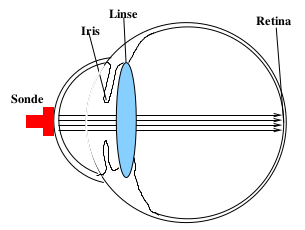
\includegraphics[scale=0.5]{auge.png}
  \caption{Augenmodell im Querschnitt \cite{anleitung}.}
  \label{fig:3}
\end{figure}
\section{Auswertung}
\subsection{Bestimmung der Schallgeschwindigkeit in Acryl}
Die aus der Messung nach dem Impuls-Echo-Verfahren gewonnenen Messwerte finden sich
in Tabelle \ref{tab:1} , die aus dem Durchschallungsverfahren in Tabelle \ref{tab:2}.
\begin{table}
  \centering
  \begin{subtable}{0.49\textwidth}
    \centering
    \begin{tabular}{c c c c}
      \toprule
      $l$/\si{\milli\metre} & $U$/\si{\volt} & $\symup{\Delta}t$/\si{\micro\second} & TGC/\si{\decibel} \\
      \midrule
      31.00 & 0.202 & 23.16 & 0 \\
      40.10 & 0.193 & 29.68 & 0 \\
      61.58 & 0.310 & 45.62 & 17.81 \\
      71.30 & - & 52.46 & 20.58 \\
      80.20 & 0.154 & 59.66 & 18.16 \\
      102.00 & 0.105 & 75.90 & 32.85 \\
      121.18 & 0.105 & 88.38 & 32.85 \\
      \bottomrule
    \end{tabular}
    \caption{Messwerte der Messung per Impuls-Echo-Verfahren. Bei den $\symup{\Delta}t$-
    Werten handelt es sich um die doppelte Laufzeit.}
    \label{tab:1}
  \end{subtable}
  \begin{subtable}{0.49\textwidth}
    \centering
    \begin{tabular}{c c c c}
      \toprule
      $l$/\si{\milli\metre} & $U$/\si{\volt} & $\symup{\Delta}t$/\si{\micro\second} & TGC/\si{\decibel} \\
      \midrule
      31.00 & 0.729 & 12.48 & 0     \\
      40.10 & 0.759 & 15.46 & 0     \\
      61.58 & 0.271 & 23.70 & 0     \\
      71.30 & -     & 27.18 & 0     \\
      80.20  & 0.154 & 30.50 & 0     \\
      102.00    & 0.271 & 38.71 & 15.48 \\
      121.18 & 0.329 & 45.19 & 17.99 \\
      \bottomrule
    \end{tabular}
    \caption{Messwerte der Messung per Durchschallungsverfahren.\\}
    \label{tab:2}
  \end{subtable}
  \caption{$l$ bezeichnet jeweils die Höhe der Zylinder, $U$ die Spannungsamplitude des
  gemessenen Peaks, $\symup{\Delta}t$ den zeitlichen Abstand zwischen senden des Schallimpulses
  und empfangen des Signals und TGC gibt den verwendeten Verstärkungsfaktor für
  den Amplitudenwert an. Die Längenmessung ist auf einen Fehler von $\pm \, \SI{0.02}{\milli\metre}$
  genau.}
\end{table}
Die Bestimmung der Schallgeschwindigkeiten gescheiht nun durch lineare Regression.
Zu beachten ist, dass sich die Laufzeiten bei der Messung per Impuls-Echo-Verfahren
Verfahrensbedingt auf die doppelte Länge beziehen. Es werden daher in den Rechnungen die halben gemessenen
Laufzeiten betrachtet.
Dies ist notwendig, da innerhalb des Sondenmaterials eine gewisse Strecke zurückgelegt werden
muss, die ansonsten als systematischer Fehler in die Rechnung eingehen würden.
Regression der Länge-Laufzeit Wertepaare mit
\begin{equation}
  t(l) = l \cdot \frac{1}{c} + t_0
\end{equation}
(wobei $c$ die Schallgeschwindigkeit im Zylinder und $t_0$ die Laufzeit innerhalb der
Sonde ist) liefert für das Impuls-Echo-Verfahren:
\begin{align*}
  c &= \SI[per-mode=reciprocal]{2740(24)}{\metre\per\second}\\
  t_0 &= \SI{0.28(25)}{\micro\second}
\end{align*}
und für das Durchschallungsverfahren:
\begin{align*}
  c &= \SI[per-mode=reciprocal]{2727(21)}{\metre\per\second}\\
  t_0 &= \SI{1.0(2)}{\micro\second}
\end{align*}
Messwerte und Regression sind in Abbildung \ref{abb:1} für das Impuls-Echo-Verfahren,
sowie in Abbildung \ref{abb:2} für das Durchschallverfahren dargestellt.
\begin{figure}
  \centering
  \begin{subfigure}{0.49\textwidth}
    \centering
    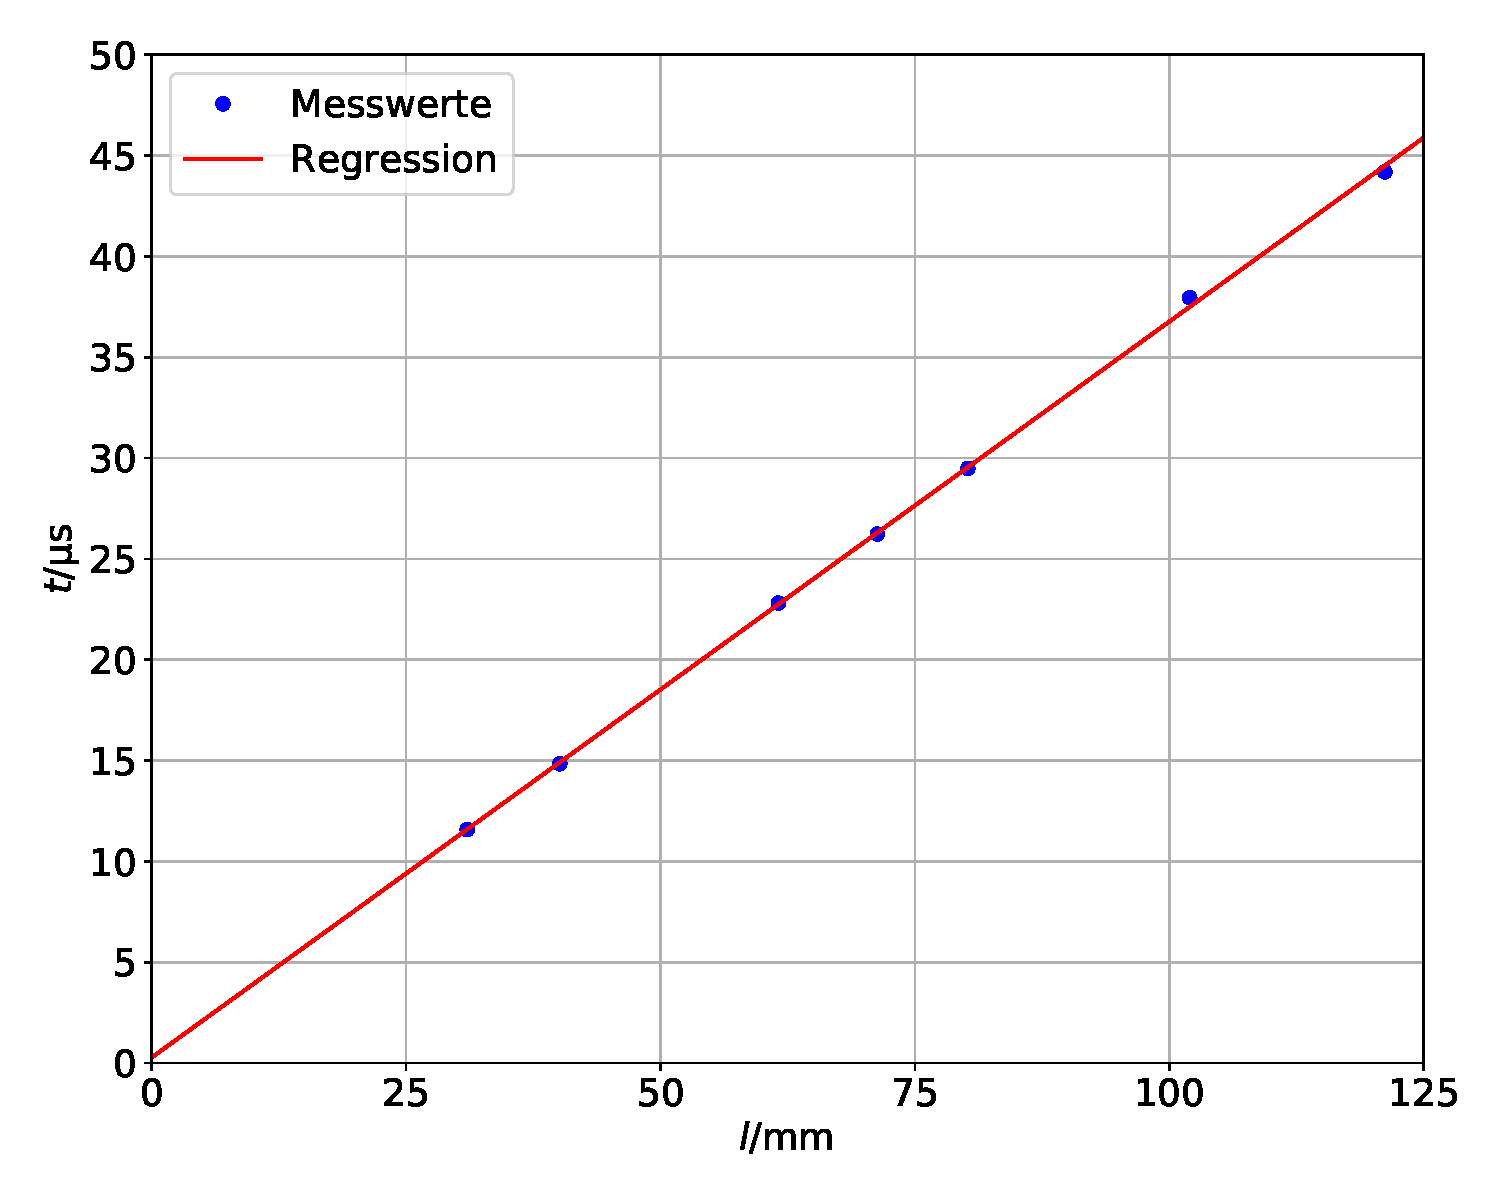
\includegraphics[width=\textwidth]{Imp.pdf}
    \caption{Impuls-Echo-Verfahren}
    \label{abb:1}
  \end{subfigure}
  \begin{subfigure}{0.49\textwidth}
    \centering
    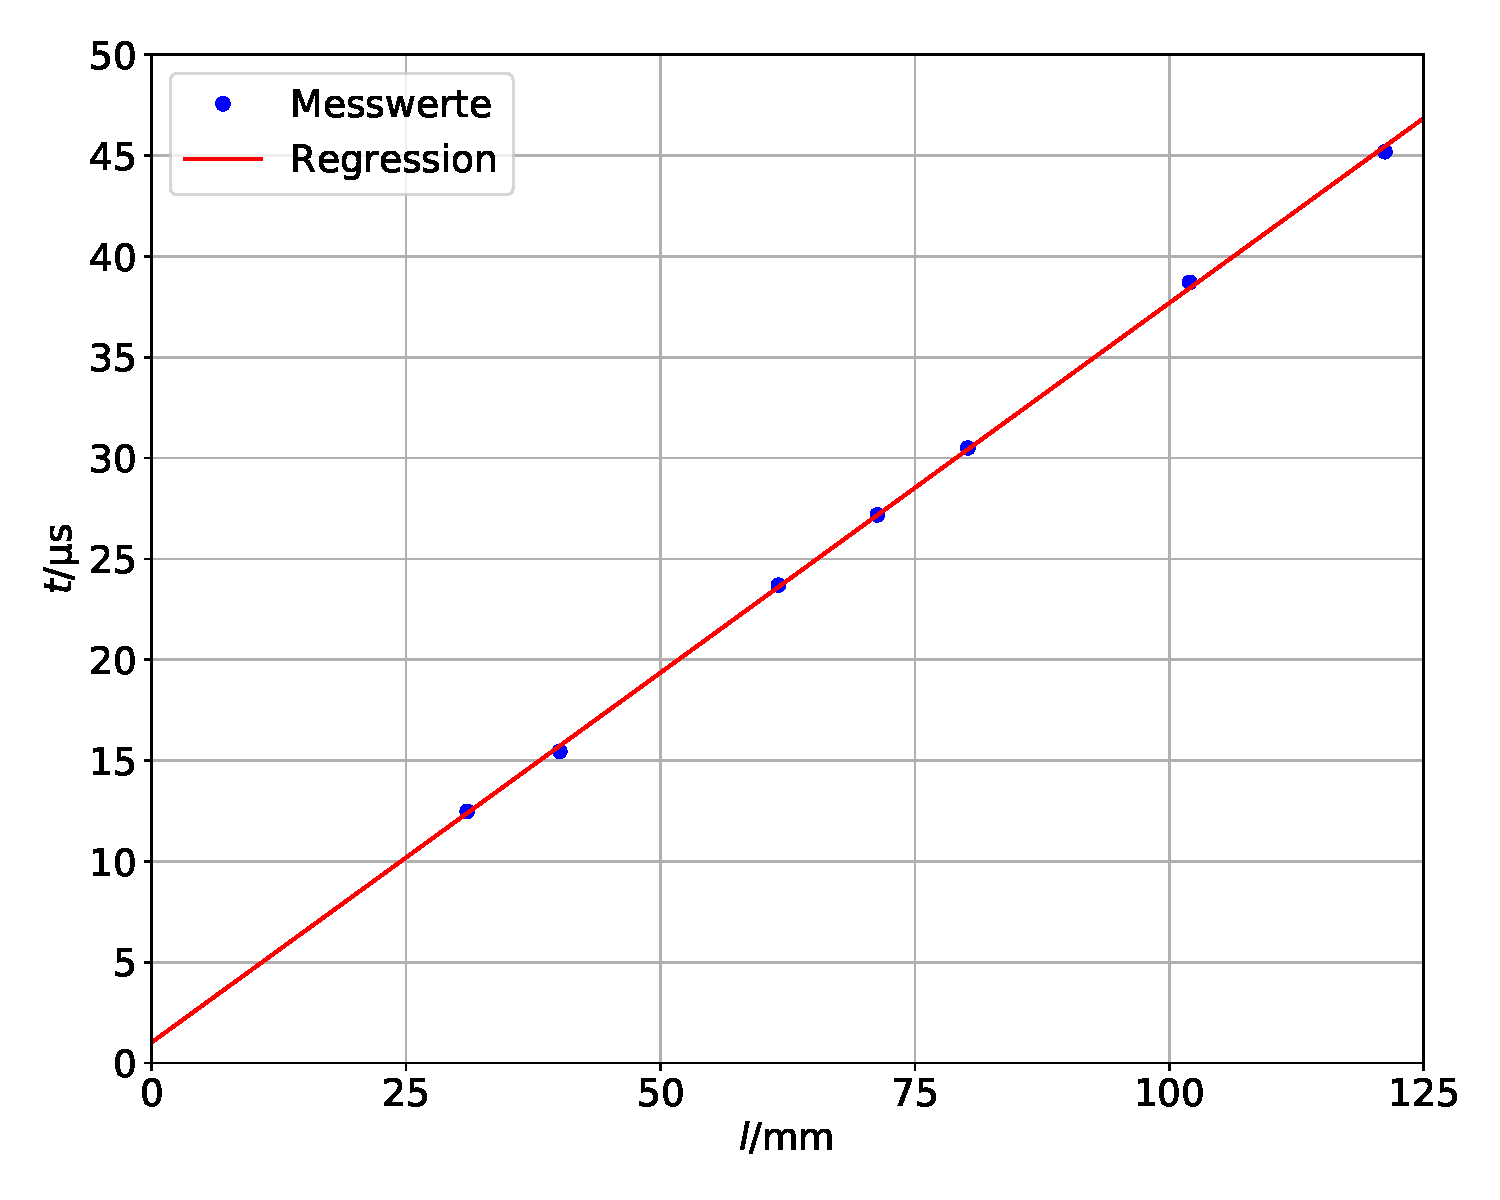
\includegraphics[width=\textwidth]{Dur.pdf}
    \caption{Durchschallverfahren}
    \label{abb:2}
  \end{subfigure}
  \caption{Dargestellt sind die gemessenen Laufzeiten bei beiden Messmethoden mit Regression.
  Insbesondere in \subref{abb:2} erkennt man die Verschiebung des Graphen auf der y-Achse,
  verursacht durch die Schalllaufzeit innerhalb der Sonde, deutlich.}
\end{figure}

\subsection{Betrachtung des Dämpfungsverhaltens von Acryl}
Nun werden die Dämpfungseigenschaften von Acryl betrachtet. Dabei wird die gemessene
Spannungsamplitude des Signals in Abhängigkeit der zurückgelegten Wegstrecke betrachtet.
Zu beachten sind hier drei Dinge:
\begin{enumerate}
  \item Beim Impuls-Echo-Verfahren wird Verfahrensbedingt die dopplete Strecke zurückgelegt.
  \item Manche Amplituden mussten mit Verstärkung gemessen werden. Diese ist in den Tabellen
  \ref{tab:1} und \ref{tab:2} als $\textsc{TGC}$-Wert in \si{\decibel} angegeben. Die Umrechnung in einen
  linearen Faktor geschieht durch:
  \begin{equation}
    G(g) = 10^{ \left( g \cdot \frac{1}{20} \right)}
    \label{eqqA:1}
  \end{equation}
  mit $\textsc{TGC}$-Wert $g$.
  \item Beim Durchschallverfahren wurde eine Empfangsverstärkung von \SI{10}{\decibel}
  zugeschaltet. Diese kann auch nach \ref{eqqA:1} eliminiert werden. Die für beide Verfahren
  genutzte Sendeverstärkung von ebenfalls \SI{10}{\decibel} verbleibt in den Messwerten,
  da sie die gesuchte Größe $\alpha$ sowie die Vergleichbarkeit beider Verfahren nicht beeinflusst.
\end{enumerate}
Die Dämpfung verläuft exponentiell, der Dämpfungskoeffizient $\alpha$ wird daher durch Regression
mit einer Funktion:
\begin{equation}
  U(l) = U_0 \cdot e^{\alpha l}
\end{equation}
in $\textsc{phyton-scipy}$ bestimmt. Zu erwähnen ist, dass die für die Zylinder mit Länge
$l=\SI{71.3}{\milli\metre}$ gemessenen Werte nicht genutzt werden können, da dieser
Zylinder aus zwei kürzeren Stücken zusammengesetzt wurde und sich so eine Signalabschwächende
Grenzschicht zwischen den beiden Zylindern bildet. Für das Impuls-Echo-Verfahren ergeben sich:
\begin{align*}
  U_0 &= \SI{0.84(33)}{\volt}\\
  \alpha &= \SI[per-mode=reciprocal]{-21(5)}{\per\metre}
\end{align*}
und für das Durchschallungsverfahren:
\begin{align*}
  U_0 &= \SI{0.69(18)}{\volt}\\
  \alpha &= \SI[per-mode=reciprocal]{-32(11)}{\per\metre}
\end{align*}
Die Verläufe mit Regression sind in den Abbildungen \ref{abb:3} und \ref{abb:4} dargestellt.
\begin{figure}
  \centering
  \begin{subfigure}{0.49\textwidth}
    \centering
    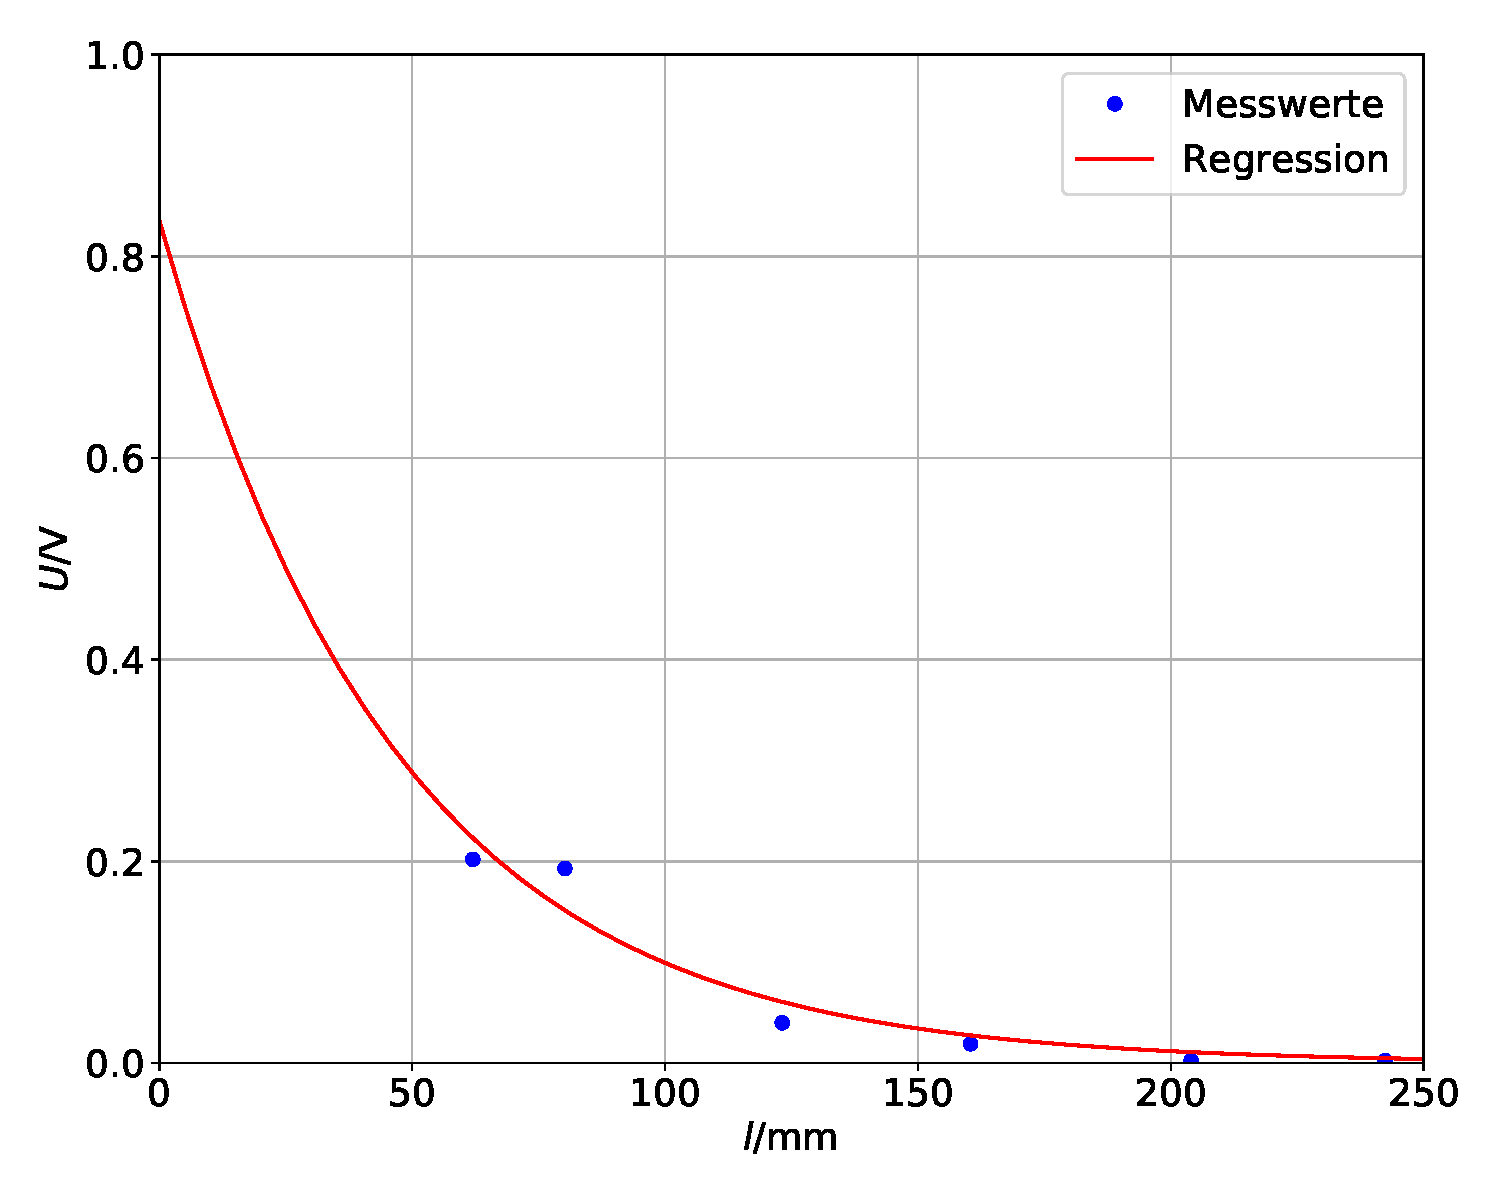
\includegraphics[width=\textwidth]{ImpDump.pdf}
    \caption{Impuls-Echo-Verfahren}
    \label{abb:3}
  \end{subfigure}
  \begin{subfigure}{0.49\textwidth}
    \centering
    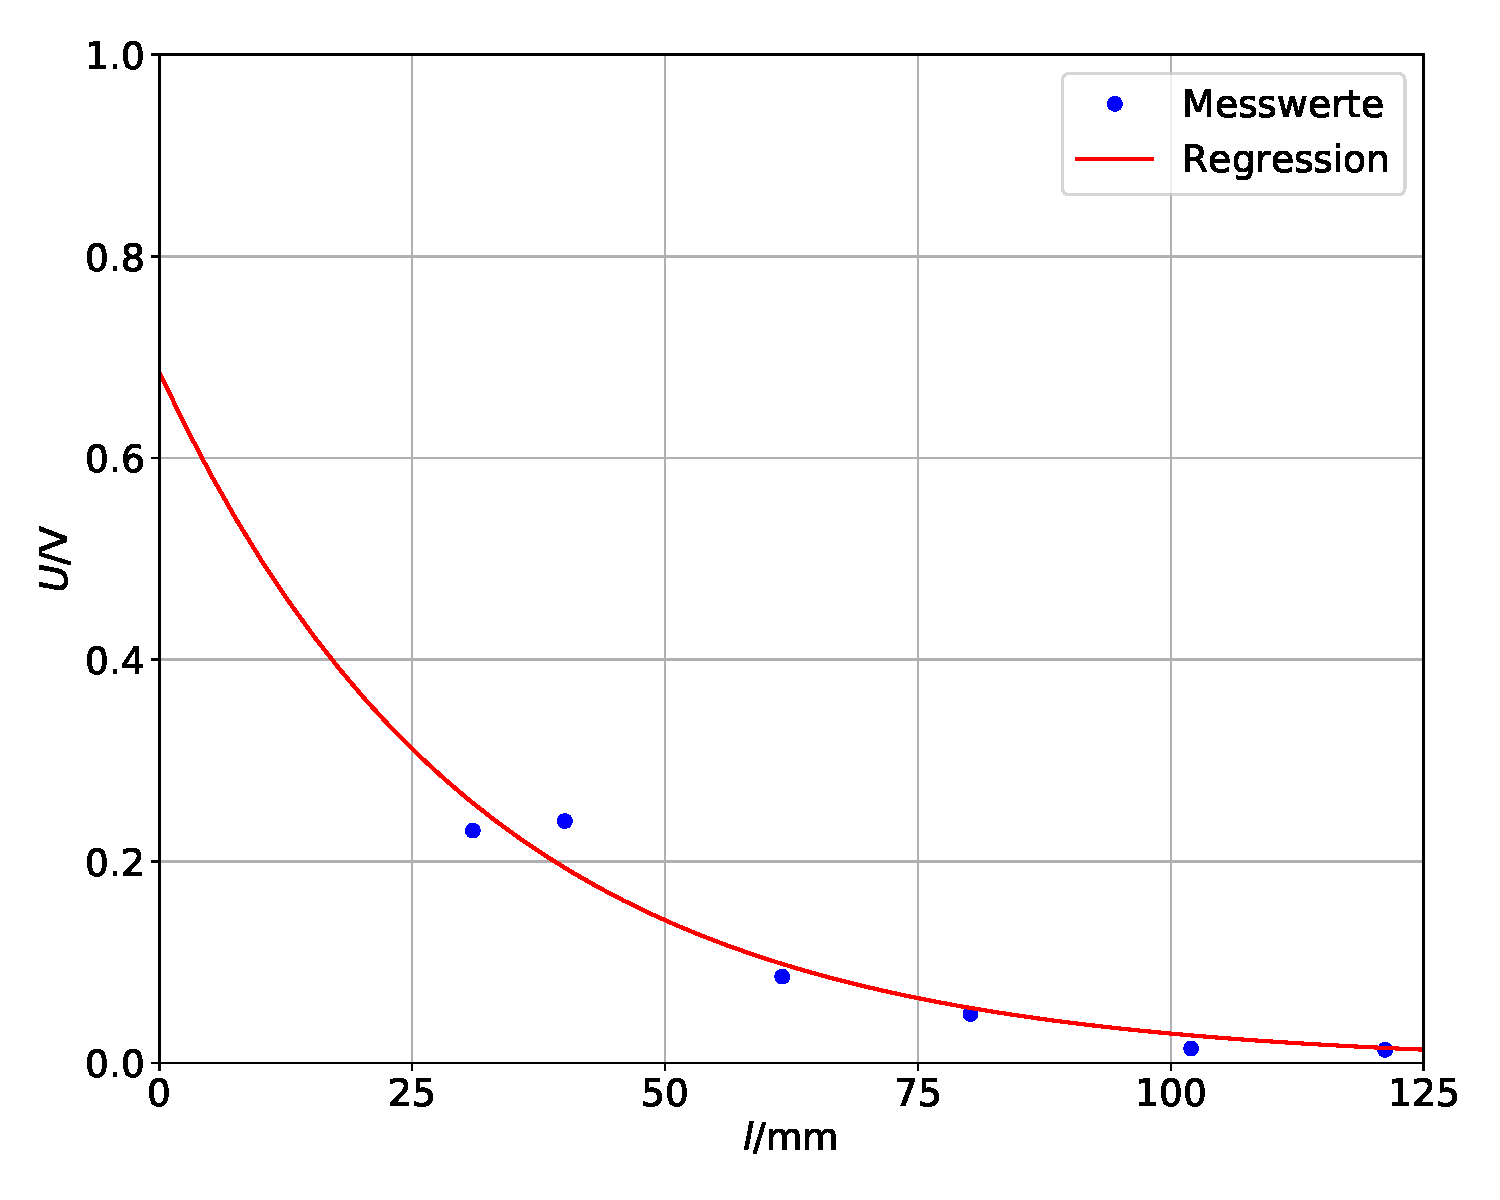
\includegraphics[width=\textwidth]{DurDump.pdf}
    \caption{Durchschallverfahren}
    \label{abb:4}
  \end{subfigure}
  \caption{Dargestellt sind die gemessenen Signalamplituden in Abhängigkeit
  der Signallaufzeit bei beiden Messmethoden mit Regression.}
\end{figure}
\subsection{Vermessung des Augenmodells}
Die gewonnen Messwerte sind in Tabelle \ref{tab:3} dargestellt. Für die Schallgeschwindigkeit\cite{anleitung}
in der Glaskörperflüssigkeit gilt $c_{GK} = \SI[per-mode=reciprocal]{1410}{\metre\per\second}$
und für die Linse $c_L = \SI[per-mode=reciprocal]{2500}{\metre\per\second}$. Sind die
Laufzeitdifferenzen $\symup{\Delta}t$ zwischen den Grenzflächen bekannt, kann nach
\begin{equation}
  S = \frac{1}{2} c \cdot \symup{\Delta}t
\end{equation}
der Abstand zwischen den Schichten bestimmt werden. Der Faktor $1/2$ ist notwending,
da beim Impuls-Echo-Verfahren die doppelten Laufzeiten gemessen werden.
\begin{table}
\begin{subtable}{0.39\textwidth}
  \centering
  \begin{tabular}{c c}
    \toprule
    Grenzschicht & $\symup{\Delta}t$/\si{\micro\second} \\
    \midrule
    Iris & 5.82 \\
    Linse ein & 10.68 \\
    Linse aus & 16.50 \\
    Retina & 69.60 \\
    \bottomrule
  \end{tabular}
  \caption{Messergebnisse.}
  \label{tab:3}
\end{subtable}
\begin{subtable}{0.59\textwidth}
  \centering
  \begin{tabular}{c c c}
    \toprule
    Grenzschicht & $l$/\si{\milli\metre} & $\frac{l}{3}$/\si{\milli\metre} \\
    \midrule
    Iris & 4.11 & 1.37\\
    Linse ein & 7.53 & 2.52\\
    Linse aus & 14.81 & 4.94\\
    Retina & 52.24 & 17.42\\
    \bottomrule
  \end{tabular}
  \caption{Berechnete Werte.}
  \label{tab:4}
\end{subtable}
\caption{Dargestellt sind in \subref{tab:3} die Ergebnisse der Vermessung des Augenmodells im Maßstab 3:1,
angegeben als Verfahrensbedingt doppelte Laufzeiten. In \subref{tab:4} finden sich
die berechnete Abstände zwischen Schallsonde und den angegebenen Grenzschichten
für das Augenmodell (Maßstab 3:1) und zurückgerechnet auf ein menschliches Auge. }
\end{table}
\subsection{Bestimmung der Dicke von Acrylplatten mithilfe des Cepstrum}
Das vermessene Cepstrum findet sich in Abbildung \ref{abb:5}, die daraus erhaltenen
Messwerte in Tabelle \ref{tab:5}.
\begin{figure}
\begin{subfigure}{0.79\textwidth}
  \centering
  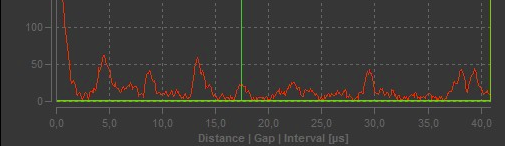
\includegraphics[width=\textwidth]{Cepstrum2.png}
  \caption{Ausschnitt des aufgenommenes Cepstrum.}
  \label{abb:5}
\end{subfigure}
\begin{subtable}{0.2\textwidth}
  \centering
  \begin{tabular}{c c }
    \toprule
    Peak & $t$/\si{\micro\second} \\
    \midrule
    1 & 4.43\\
    2 & 8.67\\
    3 & 13.19\\
    4 & 17.43\\
    \bottomrule
  \end{tabular}
  \caption{Messwerte.}
  \label{tab:5}
\end{subtable}
\caption{Das Bild des Aufgenommenen Cepstrums wurde derart beschnitten, dass die
Reflextionen der Grenzschichtend der Vorlaufstrecke nicht mitaufgenommen werden.
Ebenfalls wurde der Bereich Oberhalb von 100 Einheiten der y-Achse (im Original ebenfalls
Einheitenlos) abgeschnitten, da dort keine Informationen enthalten sind. Bei den
Messwerten in \subref{tab:5} gehören 1. und 2. sowie 3. und 4. Messwert so zusammen,
dass 3. und 4. Reflextionen von 1. und 2. sind. Wieder handelt es sich um die doppelten Werte.}
\end{figure}
Es ergeben sich also zwei Werte für die Dicke der Platten. Als Schallgeschwindigkeit wird
der aus dem Durchschallverfahren bestimmte Wert genutzt, da sein Fehlerintervall kleiner
ist. In Tabelle \ref{tab:6} sind die bestimmte Werte für die Plattendicke angegeben.
\begin{table}
\begin{subtable}{0.7\textwidth}
  \centering
  \begin{tabular}{S S S S S}
    \toprule
    \multicolumn {1}{c}{} & \multicolumn{2}{c}{Platte 1} & \multicolumn {2}{c}{Platte 2}\\
    Paar & {$\symup{\Delta}t$/\si{\micro\second}} & {$d$/\si{\milli\metre}} & {$\symup{\Delta}t$/\si{\micro\second}} & {$d$/\si{\milli\metre}} \\
    \midrule
    1 & 2.215 & \num{6.04(5)} & 4.335 & \num{11.82(9)} \\
    2 & 2.260 & \num{6.16(5)} & 4.380 & \num{11.95(9)} \\
    \bottomrule
  \end{tabular}
  \caption{Berechnete Werte.}
  \label{tab:6}
\end{subtable}
\begin{subtable}{0.29\textwidth}
  \centering
  \begin{tabular}{c c}
    \toprule
    Platte & $d$/\si{\milli\metre} \\
    \midrule
    1 & 7\\
    2 & 12\\
    \bottomrule
  \end{tabular}
  \caption{Vergleichswerte.}
  \label{tab:7}
\end{subtable}
\caption{Dargestellt sind in \subref{tab:6} die Ergebnisse für beide gemessenen Paare von Peaks.
Die Differenz $\symup{\Delta}t$ der Laufzeiten ist dabei aus den Messwerten (siehe Tabelle \ref{tab:5})
berechnet und halbiert, da die doppelte Laufzeit gemessen wurde. In \subref{tab:7} finden
sich die durch direkte Vermessung der Platten erhaltenen Werte.}
\end{table}
Die Laufzeitdifferenzen ergeben sich aus
\begin{equation}
  \symup{\Delta}t = \frac{t_2 - t_1}{2}.
\end{equation}
Wieder ist der Faktor $1/2$ notwendig, da doppelte Laufzeiten gemessen wurden. Aus
dem Wert für $\symup{\Delta}t$ lässt sich dann durch $d = ct$ der Durchmesser
der vermessenen Platte bestimmen.
\section{Diskussion}
Bei allen Messwerten ist zu beachten, dass die erhaltenen Abweichungen bei den
hohen Schallgeschwindigkeiten in den Material leicht zu großen Abweichungen führen. Dieser
Fehler wiegt insbesondere bei den letzten beiden Versuchsteilen schwer, da der erhobene
Datensatz dort extrem klein war, weshalb ein ansonsten durch die statistische Behandlung der
Daten veringerter Fehler dort ungedämpft in die Ergebnisse eingeht.
\subsection{Schallgeschwindigkeitsmessung}
Beide Ergebnisse liegen innerhalb der gegenseitigen Messungenauigkeit. Ebenfalls liegt
der Literaturwert\cite{acryl} von \SI[per-mode=reciprocal]{2730}{\metre\per\second} in den Intervallen
beider Ergebnisse. Das Fehlerintervall des durch die Durchschallungsmessung gewonnen Wertes
ist jedoch geringer als das des Wertes aus der Impuls-Echo-Methode. Dies erscheint logisch,
muss das Signal bei der Impuls-Echo-Methode den doppelten Weg zurücklegen, weshalb eventuelle
Fehler im Material einen größeren Einfluss haben und somit eine größere systematische
Fehlerquelle bieten. Auffällig ist die große Abweichung zwischen den Werten der sondeninternen
Laufzeit. Da der Fehler des bei der Messung per Impuls-Echo-Verfahren gewonnenen Wertes
jedoch annähernd so groß ist wie der Wert selbst liegt die Vermutung nah, dass hier ein
Problem vorliegt. Da jedoch beide Werte aus einer Ausgleichsrechnung mit einem sehr
begrenzten Datensatz gewonnen wurden und keine Literaturwerte vorhanden sind, kann hier nur
vermutet werden. Das aufnehmen weiterer Messwerte würde helfen, die Ergebnisse zu verifizieren.
\subsection{Dämpfungsverhalten}
Die erhaltenen Werte liegen jeweils im Bereich der gegenseitigen Messungenauigkeit.
Hohe relative Fehler der Werte lassen sich wieder durch den begrenzten Datensatz
erklären. Ebenfalls problematisch sind die langen Laufzeiten bei der Impuls-Echo-Messung.
Die erhaltenen Daten sind daher bereits stärker gedämpft, weshalb die Ausgleichsrechnung
statisch signifikantere Fehler ergeben sollte. Ein Literaturwert\cite{daempf} von \SI{1.41}{\per\centi\metre}
liegt in keinem der beiden Fehlerintervalle. Auch die relativen Fehler sind mit \SI{85}{\percent}
für die Durchschallungsmessung sowie \SI{77}{\percent} sehr hoch. Der Schluss eines
systematischen Fehlers liegt nahe.
\subsection{Messung am Augenmodell}
Für das Augenmodell ergeben sich realistische Werte. Der Durchmesser eines Menschlichen
Auges liegt laut Literatur\cite{auge} zwischen \SI{17}{\milli\metre} und \SI{30}{\milli\metre},
je nach Alter des betrachteten Präparates. Der ermittelte Werte trifft daher auf das Auge eines
Kleinkindes zu.
\subsection{Dickenbestimmung per Cepstrum}
Im Vergleich mit den durch direkte Vermessung erhaltenen Werten zeigen sich Abweichungen.
Lediglich bei einem der vier Werte liegt der Vergleichswert im Fehlerintervall. Die maximale relative
Abweichung ist mit \SI{0.96}{\milli\metre} (dies entspricht \SI{13}{\percent}) jedoch
vergleichsweise gering. Insbesondere bei den in Acryl vorhandenen hohen Schallgeschwindigeiten
kann dies leicht zu großen Abweichungen führen.



\newpage
\nocite{*}
\printbibliography
